\documentclass[tikz,border=12pt]{standalone}
\usepackage{amsmath,amssymb}
\usetikzlibrary{calc}

\begin{document}
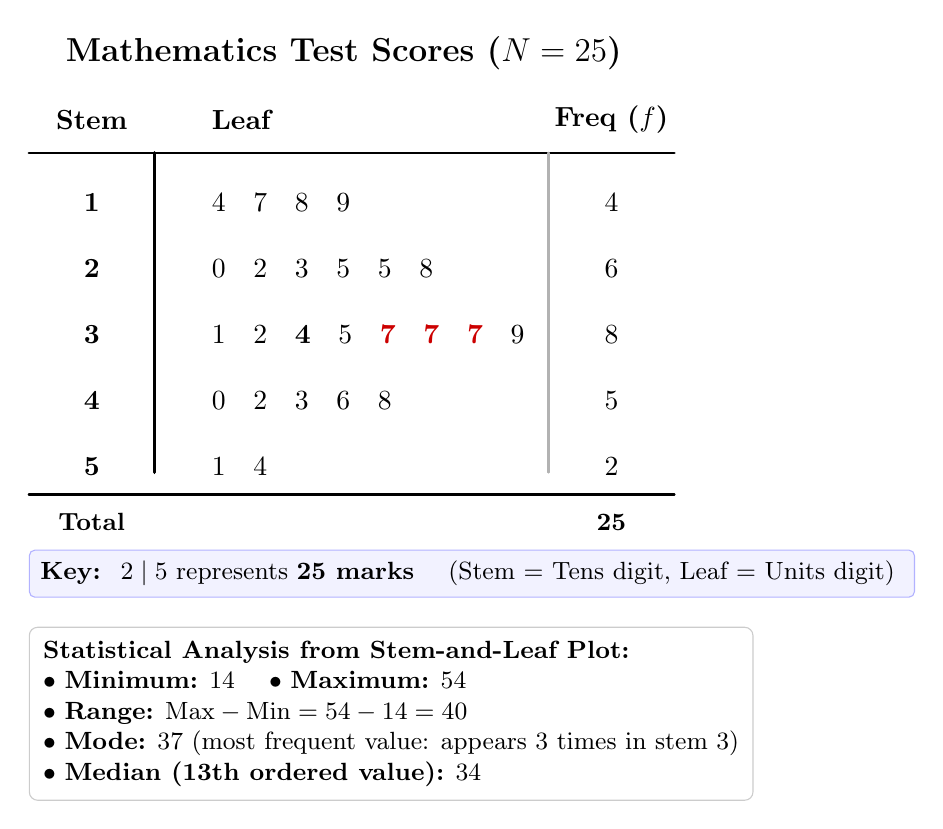
\begin{tikzpicture}[x=1cm, y=0.7cm, line cap=round, line join=round]

  % Title banner
  \node[font=\large\bfseries] at (4.0, 7.2) {Mathematics Test Scores ($N = 25$)};

  % Header row (y = 6)
  \node[font=\normalsize\bfseries] at (0.8, 6.0) {Stem};
  \node[font=\normalsize\bfseries, anchor=west] at (2.2, 6.0) {Leaf};
  \node[font=\normalsize\bfseries] at (7.4, 6.0) {Freq ($f$)};

  % Horizontal dividing line under header
  \draw[thick] (0, 5.4) -- (8.2, 5.4);

  % Vertical dividing rule between Stem and Leaf
  \draw[very thick] (1.6, 5.4) -- (1.6, -0.4);
  % Vertical dividing rule between Leaf and Frequency (moved to 6.6 for ample clearance)
  \draw[thick, gray!60] (6.6, 5.4) -- (6.6, -0.4);

  % Data Rows
  % Row 1: Stem 1 (y = 4.5)
  \node[font=\normalsize\bfseries] at (0.8, 4.5) {1};
  \node[font=\normalsize, anchor=west] at (2.2, 4.5) {4 \ \ 7 \ \ 8 \ \ 9};
  \node[font=\normalsize] at (7.4, 4.5) {4};

  % Row 2: Stem 2 (y = 3.3)
  \node[font=\normalsize\bfseries] at (0.8, 3.3) {2};
  \node[font=\normalsize, anchor=west] at (2.2, 3.3) {0 \ \ 2 \ \ 3 \ \ 5 \ \ 5 \ \ 8};
  \node[font=\normalsize] at (7.4, 3.3) {6};

  % Row 3: Stem 3 (y = 2.1)
  \node[font=\normalsize\bfseries] at (0.8, 2.1) {3};
  \node[font=\normalsize, anchor=west] at (2.2, 2.1) {1 \ \ 2 \ \ \textbf{4} \ \ 5 \ \ \textcolor{red!80!black}{\textbf{7}} \ \ \textcolor{red!80!black}{\textbf{7}} \ \ \textcolor{red!80!black}{\textbf{7}} \ \ 9};
  \node[font=\normalsize] at (7.4, 2.1) {8};

  % Row 4: Stem 4 (y = 0.9)
  \node[font=\normalsize\bfseries] at (0.8, 0.9) {4};
  \node[font=\normalsize, anchor=west] at (2.2, 0.9) {0 \ \ 2 \ \ 3 \ \ 6 \ \ 8};
  \node[font=\normalsize] at (7.4, 0.9) {5};

  % Row 5: Stem 5 (y = -0.3)
  \node[font=\normalsize\bfseries] at (0.8, -0.3) {5};
  \node[font=\normalsize, anchor=west] at (2.2, -0.3) {1 \ \ 4};
  \node[font=\normalsize] at (7.4, -0.3) {2};

  % Bottom rule
  \draw[thick] (0, -0.8) -- (8.2, -0.8);

  % Total row (y = -1.3)
  \node[font=\small\bfseries] at (0.8, -1.3) {Total};
  \node[font=\small\bfseries] at (7.4, -1.3) {25};

  % Key / Legend Card (y = -1.8)
  \node[align=left, font=\small, fill=blue!5, inner sep=4pt, draw=blue!30, rounded corners=2pt, anchor=north west] at (0, -1.8) {
    \textbf{Key:} \ $2 \mid 5$ represents \textbf{25 marks} \quad (Stem = Tens digit, Leaf = Units digit)
  };

  % Statistical Summary Card below (y = -3.2)
  \node[align=left, font=\small, fill=white, inner sep=5pt, draw=gray!40, rounded corners=3pt, anchor=north west] at (0, -3.2) {
    \textbf{Statistical Analysis from Stem-and-Leaf Plot:}\\
    $\bullet$ \textbf{Minimum:} $14$ \quad $\bullet$ \textbf{Maximum:} $54$\\
    $\bullet$ \textbf{Range:} $\text{Max} - \text{Min} = 54 - 14 = 40$\\
    $\bullet$ \textbf{Mode:} $37$ (most frequent value: appears 3 times in stem 3)\\
    $\bullet$ \textbf{Median (13th ordered value):} $34$
  };

\end{tikzpicture}
\end{document}
